\documentclass[border=10pt]{standalone}
\usepackage{pgfplots}
\usepackage{siunitx}
\pgfplotsset{width=7cm,height=7cm,compat=1.8}
\usepgfplotslibrary{polar}

\pgfplotsset{myplot/.style={%
  clip=false, % needed for double line (last \addplot command)
  domain=-pi/2:3/2*pi, % plot full cycle
  samples=1000, % number of samples; can be locally adjusted
  grid=none, % display major and minor grids
  xtick={-pi/2,0,...,pi/2*3},
  xtick align=outside,
  xticklabels={%
  $-\pi/2$,  
  $0$,  
  $\pi/2$,
    $\pi$,
    $3\pi/2$
  },
  xmin=-pi/2,
xmax=3/2*pi,
ymin=0,
ymax=1,
  major grid style={black}, 
  yticklabel style={anchor=east}, % move label position
}}

\pgfplotsset{mypolarplot/.style={%
  clip=false, % needed for double line (last \addplot command)
  domain=0:180, % plot full cycle
  samples=101, % number of samples; can be locally adjusted
  grid=both, % display major and minor grids
  major grid style={black}, 
  minor x tick num=3, % 3 minor x ticks between majors
  minor y tick num=1, % 1 minor y tick between majors
  xtick={0,90,...,359},
  xticklabels={%
    $\theta = \ang{0}$,
    $\theta = \ang{90}$,
    $\theta = \ang{180}$,
    $\theta = \ang{270}$
  },
  yticklabel style={anchor=north east}, % move label position
}}

\begin{document}



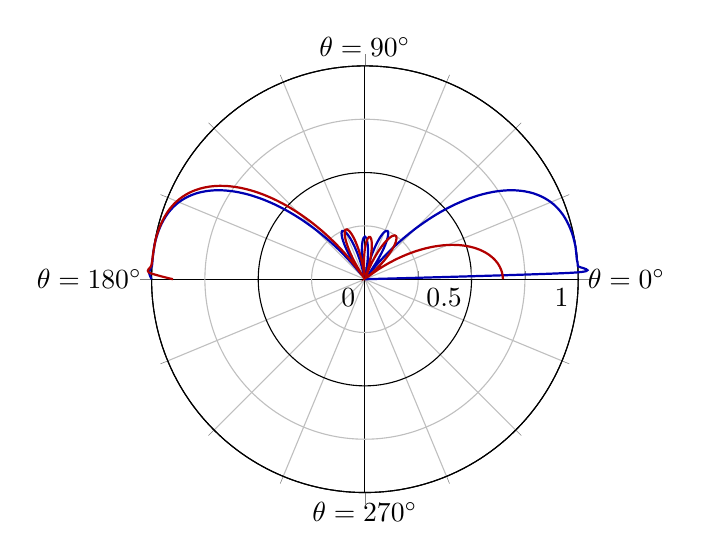
\begin{tikzpicture}

      \pgfmathsetmacro{\alphaa}{180}
      \pgfmathsetmacro{\da}{1/2}
      \pgfmathsetmacro{\alphab}{0.9*180}
      \pgfmathsetmacro{\db}{.45}
      \pgfmathsetmacro{\N}{5}
      \begin{polaraxis}[%
        ymax=1,
        ytick={0,.5,1},
        mypolarplot,legend style={at=(current axis.south east), anchor=south west}
      ]

      \addplot[mark=none,blue!70!black,thick] plot[smooth] 
      {1/\N*abs(sin(\N/2*(2*180*\da*cos((\x))+\alphaa))/sin((2*180*\da*cos((\x))+\alphaa)/2))};


      \addplot[mark=none,red!70!black,thick] plot[smooth] 
      {1/\N*abs(sin(\N/2*(2*180*\db*cos((\x))+\alphab))/sin((2*180*\db*cos((\x))+\alphab)/2))};
      
      \end{polaraxis}
\end{tikzpicture}
\end{document}